
\documentclass[11pt]{article}


\usepackage[left=1in,top=1in,right=1in,bottom=1in,nohead]{geometry}
\usepackage{graphicx,url}
\usepackage{siunitx,multirow}
\usepackage{amsmath,amsfonts,amssymb,multicol}
\usepackage{algorithmic,algorithm,titlesec}
\usepackage{setspace}

 \titleformat{\section}{\normalfont\normalsize\bfseries}{\thesection.}{1mm}{ }
\titleformat{\subsection}{\normalfont\normalsize\itshape}{\thesubsection.}{1mm}{}
  
 \titlespacing{\section}{0pt}{3pt}{0pt}
\titlespacing{\subsection}{0pt}{3pt}{0pt}

\setlength{\parindent}{3mm} % size of subsequent paragraph indents 
                          
 \renewenvironment{abstract}
 {\par\noindent\textbf{\abstractname.}\ \ignorespaces}
 {\par\medskip}   
                       

\begin{document}

\title{\large {\bf Time-Frequency Analysis of Signals}\\[2mm]
Project Final Report, EEE 505 Spring 2022}

\author{\large  Stud E. NtA and Stud E. NtB}
\date{ } 

\maketitle

\doublespacing

\begin{abstract}
Each paper must include an abstract of 100-150 words.
Some directions on how to write an abstract can be found on Canvas
under  the Course Project module. 
\end{abstract}

\section{Some Information}
\label{sec:info}

The provided \LaTeX \ template sets  the required line spacing to double, font size to 11 point,
 and margins to one inch on each side.   Note that any equation, figure, table, or 
 algorithm  you provide must be  discussed in the report.  For example, 
the Wigner distribution (WD) time-frequency  representation (TFR)  is defined as  \cite{Hla92,Mal93}
 \begin{equation}
\int_{-\infty}^{\infty} W_x(t, f)  \, \delta (f - \alpha t ) \, df =    W_x(t, \alpha t ) \, ,
\label{eq:WD}
\end{equation}
where  $x(t)$ is the analysis signal and 
$\alpha$  is the frequency-modulation  rate in  Hz$^2$.  

 \section{Some Other Information}
 
Table \ref{table1} has multiple columns, and  Figure \ref{fig} 
shows the scalogram TFR of the sum of two  sinusoids. 
Algorithm \ref{alg1} summarized some computation steps, and in 
  Section \ref{sec:info},    Equation \eqref{eq:WD} should look familiar.
 Appendix A provides some directions, if needed,  on how to include  {\sc Matlab} code.
 
\begin{table}[h]
\begin{center}
   \begin{tabular}{| l | c | c | r| }  \hline 
   \textbf{Header 1} & \textbf{Header 2} & \textbf{Header 3} & \textbf{Header 4} \\[1mm]  \hline
   \multicolumn{3}{|c}{Multiple Column Entry} & Item 4 \\
1  &  2 &  3 &  4\\ \hline 
   \end{tabular}
   \end{center}
    \caption{Table with multiple columns.} 
   \label{table1}
\end{table}

\subsection{More related information}

This bibliography is generated using  {\sc BibTeX}  
 (see \url{http://www.bibtex.org/}).  There are references for 
 a book   \cite{The20} and a  conference paper  \cite{Veg14}.


\begin{figure}[t]
\begin{center}
\resizebox{!}{2.5in}{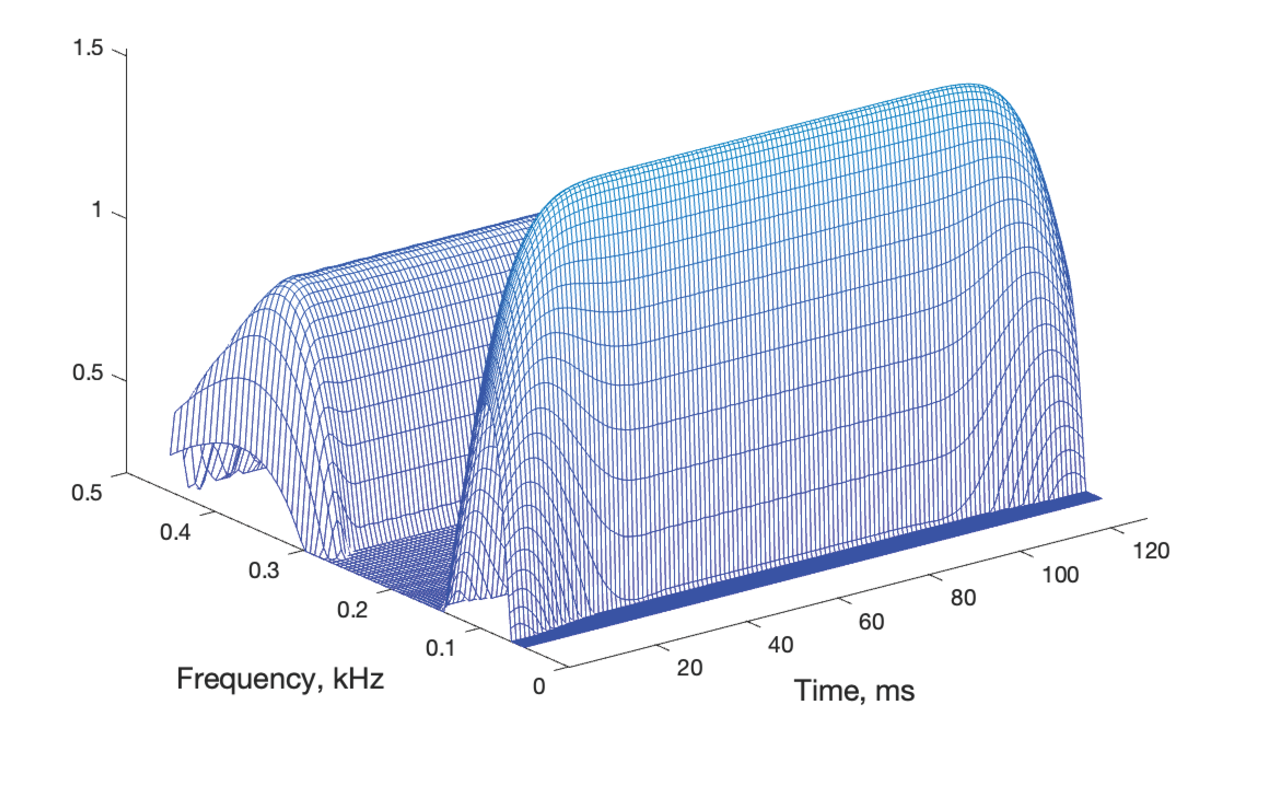
\includegraphics{figure1.eps}}
\end{center}
\caption{Scalogram of the sum of  two signals,  a 100 Hz sinusoid 
and  350 Hz  sinusoid.}
\label{fig}
\end{figure}

\begin{algorithm}[h] 
\caption{Some steps.}
\begin{algorithmic}
%
\STATE Input: sampling period $T_s$, signal $x(t)$ 
\STATE Obtain signal samples  $x[n]=x(n  T_s)$        
 \FOR{$n=1$  \TO $30$}
%
\STATE  $z[n]=y[n-1]$
\ENDFOR
\STATE Output: signal $z[n]$
%
\end{algorithmic}
\label{alg1}
\end{algorithm}

\begin{singlespace}
 \titlespacing{\section}{0pt}{12pt}{12pt}
 
\bibliographystyle{ieeetr}
\bibliography{refs_FinalRept.bib}
\end{singlespace}

\section*{Appendix A: Matlab Code}

  {\sc Matlab} code can only be provided in an appendix and only if you wrote it.
If the code is not original,  you must provide its source.
To include code, you could use the   {\tt mcode} package or  the latex command {\tt verbatim}.


\end{document}